\documentclass{UNESC}
\usepackage[T1]{fontenc}
\usepackage[utf8]{inputenc}%\usepackage[latin1]{inputenc}
\renewcommand{\rmdefault}{phv} % Arial
\renewcommand{\sfdefault}{phv} % Arial
\usepackage[brazilian]{babel}
\usepackage{graphicx}
\usepackage{hyperref}
\usepackage{quoting}
\usepackage[labelsep=none]{caption}
\DeclareCaptionLabelFormat{figuracomtraco}{#1~#2 -}
\captionsetup[figure]{labelformat=figuracomtraco, labelsep=space}
\captionsetup[table]{labelformat=simple, labelsep=space, textformat=simple}
\DeclareCaptionLabelFormat{tabelacomtraco}{#1~#2 -}
\captionsetup[table]{labelformat=tabelacomtraco}
\captionsetup{labelsep=none}
\captionsetup[table]{format=hang,justification=raggedright,
  singlelinecheck=false,labelsep=space,font=normalsize,
  labelfont=normalfont,textfont=normalfont,skip=6pt}
\usepackage{enumitem}
\usepackage{float}
\usepackage{comment}
\usepackage[hang,flushmargin]{footmisc}
\usepackage{array}
\usepackage{adjustbox}
\setlength{\emergencystretch}{3em}

\hypersetup{
  setpagesize  = false,
  colorlinks   = true,
  urlcolor     = blue,
  linkcolor    = black,
  citecolor    = black
}

\urlstyle{same}
\usepackage{setspace}

\usepackage[alf,recuo=0.0cm,abnt-emphasize=bf]{abntex2cite} 

\title{REGISTRO DIGITAL ANIMAL: DIGITALIZANDO A IDENTIFICAÇÃO E CONTROLE DE VACINAÇÃO DE ANIMAIS DE ESTIMAÇÃO}
\author
{
   Gabriel Goulart de Souza\footnote{Curso de Ciência da Computação, Universidade do Extremo Sul Catarinense (Unesc), Criciúma - Santa Catarina - Brasil. gabriel.gsouzza6@unesc.net},
   Diorgines Mattos Machado\footnote{Coorientador(a), Curso de Ciência da Computação, Universidade do Extremo Sul Catarinense (Unesc), Criciúma - Santa Catarina - Brasil. diorginesmattos@unesc.net},
   Allan Farias Favaro\footnote{Orientador(a), Curso de Ciência da Computação, Universidade do Extremo Sul Catarinense (Unesc), Criciúma - Santa Catarina - Brasil. allanfavaro@gmail.com}
}

% Limite obrigatório: PDF completo com 20 páginas ou menos, incluindo referências.
\begin{document}

\onehalfspacing

\maketitle

\noindent
\textbf{Resumo:} A dispersão de dados de identificação, vacinação e documentos clínicos dificulta a organização do histórico de animais de estimação. Este trabalho teve como objetivo desenvolver e avaliar o funcionamento de uma aplicação multiplataforma para cadastrar, organizar e consultar esses registros. A aplicação Registro Digital Animal foi desenvolvida como aplicação web progressiva, com autenticação, sincronização e persistência no PostgreSQL. A avaliação reuniu 15 cenários funcionais de caixa-preta, dois retornos preservados do setor veterinário e uma coleta complementar com cinco envios de quatro contas. Nesta última, um envio repetido foi desconsiderado, resultando em quatro avaliações e 24 respostas a afirmações de concordância. Os cenários funcionais foram registrados como aprovados nas condições avaliadas. Os retornos anteriores apontaram utilidade na organização dos dados e dificuldades de preenchimento. Nos novos registros, três contas concordaram parcial ou totalmente com a utilidade de alertas vacinais e de checklist por pet, enquanto uma discordou totalmente. Os comentários orientaram a implementação de avisos internos, resumo de vacinas vencidas, planejamento de viagens com vários pets e itens adicionais no checklist, acompanhados de testes técnicos. A contribuição consiste no artefato e na rastreabilidade entre necessidades relatadas e alterações implementadas. O conjunto reduzido, a caracterização incompleta das contas e a ausência de reavaliação das melhorias impedem generalizar a usabilidade ou atribuir benefícios clínicos. A redução do uso de documentos físicos não foi mensurada.

\vspace{0.5em}
\noindent
\textbf{Palavras-chave:} animais de estimação; registro digital; vacinação animal; aplicação web progressiva; testes funcionais.

\vspace{1.0em}
\noindent
\textbf{ABSTRACT:} Scattered identification, vaccination and clinical documents make it difficult to organize companion animals' records. This study aimed to develop and evaluate the operation of a cross-platform application for registering, organizing and consulting these records. Registro Digital Animal was developed as a progressive web application with authentication, synchronization and PostgreSQL persistence. The evaluation combined 15 black-box functional scenarios, two preserved responses from the veterinary sector and an additional collection comprising five submissions from four accounts. One repeated submission was excluded from the latter analysis, yielding four assessments and 24 responses to agreement statements. The functional scenarios were recorded as passed under the evaluated conditions. Earlier responses indicated usefulness in organizing records and difficulties entering information. In the additional collection, three accounts partly or fully agreed that vaccination alerts and per-pet checklists would be useful, while one fully disagreed. Comments informed the implementation of in-app reminders, an overdue-vaccination summary, multi-pet travel planning and additional checklist items, supported by technical tests. The contribution comprises the software artifact and traceability between reported needs and implemented changes. The small dataset, incomplete account characterization and lack of post-change evaluation prevent generalizing usability or attributing clinical benefits. A reduction in the use of physical documents was not measured.

\vspace{0.5em}
\noindent
\textbf{Keywords:} companion animals; digital records; animal vaccination; progressive web application; functional testing.

\section{INTRODUÇÃO}

A consolidação da família multiespécie ampliou a importância dos animais de estimação no núcleo familiar e a preocupação dos tutores com sua saúde e bem-estar \cite{BOLSON2022,VIEIRA2020}. Esse contexto exige organizar informações de identificação e saúde, para as quais aplicativos e sistemas veterinários oferecem alternativas de registro e consulta \cite{MORAES2024}. A identificação individual também contribui para o acompanhamento do comportamento e das condições dos animais \cite{vidal2021}.

Dados de vacinação, exames, consultas e medicamentos compõem o histórico de saúde. A identificação e a rastreabilidade auxiliam o monitoramento e o controle de doenças infecciosas e zoonoses \cite{murphy2008}, enquanto a vacinação constitui medida preventiva relevante, inclusive contra a raiva \cite{MOUTINHO2017}. Entretanto, cadernetas e fichas em papel estão sujeitas a perdas, danos e deterioração \cite{BOLSON2022}, dificultando a consulta em atendimentos, viagens ou emergências. A digitalização foi adotada neste trabalho para reunir esses registros em um ambiente consultável pelo tutor.

Soluções existentes apresentam focos distintos. Prontuários eletrônicos veterinários demonstram a viabilidade da informatização, mas se dirigem principalmente às clínicas \cite{iskandar2023}. Plataformas de cadastro e controle de vacinação centralizam serviços, mantendo oportunidades relacionadas à mobilidade e ao acesso sem internet \cite{vieira2025}. A comunicação por aproximação complementa métodos tradicionais de identificação \cite{sartori2018}, e a rastreabilidade permite acompanhar origem, movimentações e registros sanitários \cite{zhao2020}. Isoladamente, essas tecnologias não reúnem necessariamente os documentos utilizados pelo tutor no cotidiano.

Essa diversidade de propostas permite delimitar o problema: informações de identificação, vacinação e documentos clínicos podem permanecer distribuídas entre papéis, estabelecimentos e sistemas. A proposta se justifica pela necessidade de organizá-las em uma interface acessível ao tutor, considerando mobilidade, consulta local e continuidade do acesso. No domínio computacional, o trabalho aplica desenvolvimento multiplataforma, modelagem relacional e mecanismos de persistência e sincronização.

Apresenta-se, assim, a aplicação \textbf{Registro Digital Animal}, com arquitetura de \textit{Progressive Web App} (PWA), acesso pelo navegador e instalação no dispositivo. O \textit{cache} e a persistência local permitem consultar dados previamente armazenados sem conexão. O objetivo geral foi desenvolver e avaliar o funcionamento de uma aplicação multiplataforma para cadastrar, organizar e consultar registros de identificação, vacinação e documentos clínicos de animais de estimação. A redução da dependência de documentos físicos é um benefício pretendido, não mensurado neste estudo.

\section{MATERIAIS E MÉTODOS}

A pesquisa é aplicada, pois buscou uma solução tecnológica para um problema prático de gerenciamento de informações de saúde e identificação de animais de estimação. Tem abordagem qualitativa e caráter exploratório e descritivo, ao investigar as tecnologias empregadas na digitalização de registros veterinários e descrever o desenvolvimento e a modelagem da aplicação. O estudo foi orientado pela construção e avaliação de um artefato computacional, em aproximação à \textit{Design Science Research} (DSR), que relaciona a identificação de um problema à definição de objetivos, ao desenvolvimento e à avaliação de uma solução \cite{peffers2007}. Aqui, o problema foi delimitado pela organização e consulta dos registros dos animais; os requisitos foram materializados nos módulos de cadastro, carteira, vacinação, documentos e acesso local; o artefato foi implementado como aplicação multiplataforma; e sua avaliação foi feita por cenários funcionais e retornos de participantes do setor veterinário. Esse encadeamento descreve apenas as atividades documentadas, sem pressupor etapas adicionais ou ciclos experimentais não registrados.

\subsection{Desenvolvimento do Sistema}

O desenvolvimento produziu a aplicação Registro Digital Animal, voltada ao uso cotidiano do tutor. Os requisitos contemplam cadastro de usuários e animais, organização de vacinas e documentos, carteira digital, planejamento de viagens e consulta de estabelecimentos veterinários, com interface para computadores e dispositivos móveis, persistência local e sincronização com o servidor. O código-fonte está em repositório público\footnote{Disponível em: \url{https://github.com/Gabriel-GDS-dev/PetIdentification}. Acesso em: 28 out. 2026.}.

\subsubsection{Arquitetura e Tecnologias do Sistema}

O sistema adota arquitetura cliente-servidor, separando a interface, o processamento das requisições e a persistência dos dados: uma \textit{Progressive Web App} (PWA) no \textit{frontend}, uma API REST no \textit{backend} e um banco relacional PostgreSQL 18, além de serviços externos em funcionalidades específicas. A Figura~\ref{fig:fluxograma_sistema} sintetiza a interação entre usuário, interface, serviços, banco de dados e recursos externos. O tutor acessa a aplicação pelo navegador ou pela PWA instalada; as ações são encaminhadas à API REST, que aplica as regras do sistema e opera o banco, enquanto o armazenamento local e a sincronização mantêm as informações essenciais disponíveis com conectividade limitada ou ausente.

\begin{figure}[htbp]
\captionsetup{justification=raggedright,singlelinecheck=false,format=hang}
\caption[Fluxograma da arquitetura e do funcionamento do sistema Registro Digital Animal]{Fluxograma da arquitetura e do funcionamento do sistema \mbox{Registro Digital Animal}}
\label{fig:fluxograma_sistema}
\centering
\vspace{-0.2cm}
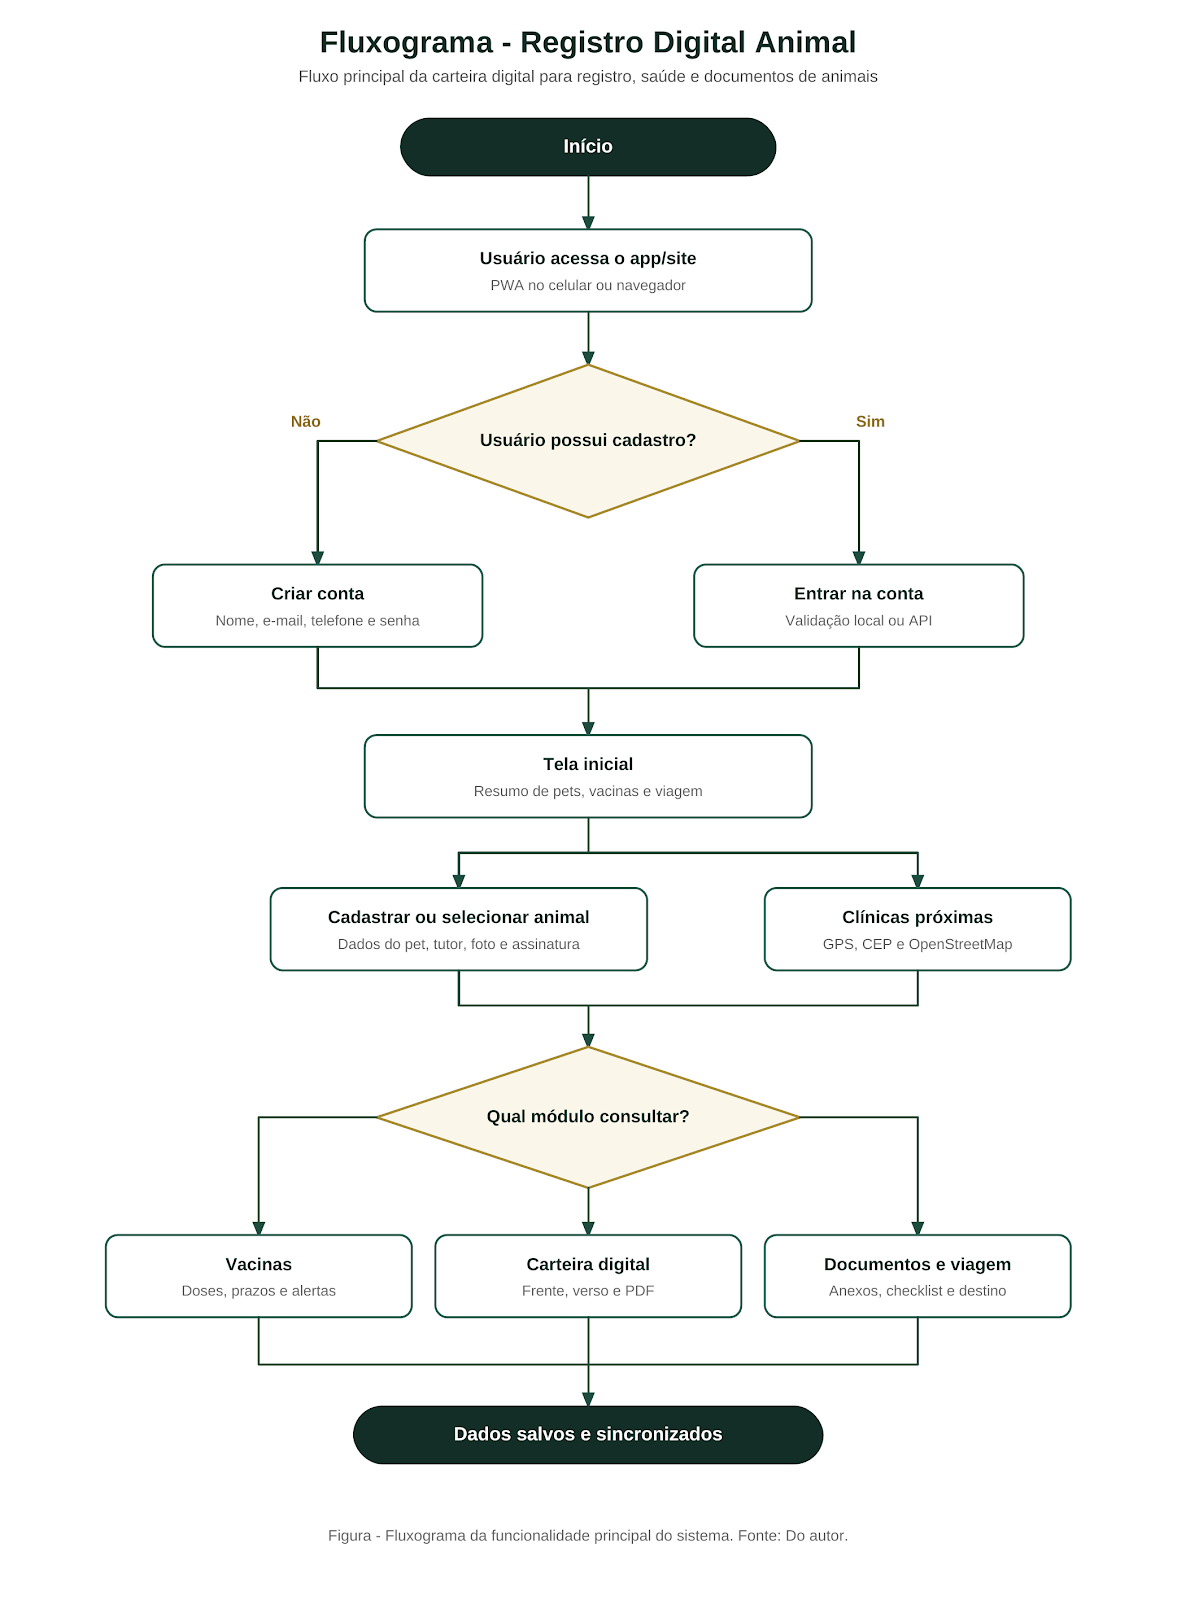
\includegraphics[scale=0.2]{Figs/fluxograma-registro-digital-animal.png}

\vspace{-0.2cm}
\begin{minipage}{\textwidth}
\footnotesize\raggedright Fonte: Elaborado pelo autor com auxílio do Codex GPT-5.5 (2026).
\end{minipage}
\end{figure}

A Figura~\ref{fig:arquitetura_tecnologias_sistema} apresenta as tecnologias por camada. No \textit{frontend}, são usados HTML5, CSS3 e JavaScript puro, com manifesto, \textit{service worker}, \textit{cache} e armazenamento local para os recursos de PWA. O \textit{backend} é escrito em JavaScript sobre Node.js, organizado como API REST, com NPM no gerenciamento das dependências. A persistência usa PostgreSQL 18, com conexão parametrizada por variáveis de ambiente. A infraestrutura da etapa de avaliação utilizou Render Postgres e Render Web Service, e o projeto também contém configuração para publicação na Vercel e execução local. A coleta complementar de novembro utilizou PostgreSQL pela integração Prisma Postgres da Vercel, distinguindo-se da infraestrutura inicial. A indisponibilidade posterior do banco hospedado limitou a recuperação de parte dos retornos da pesquisa de campo, como descrito adiante.

\begin{figure}[htbp]
\captionsetup{justification=raggedright,singlelinecheck=false,format=hang}
\caption{Arquitetura e tecnologias utilizadas no sistema Registro Digital Animal}
\label{fig:arquitetura_tecnologias_sistema}
\centering
\vspace{-0.2cm}
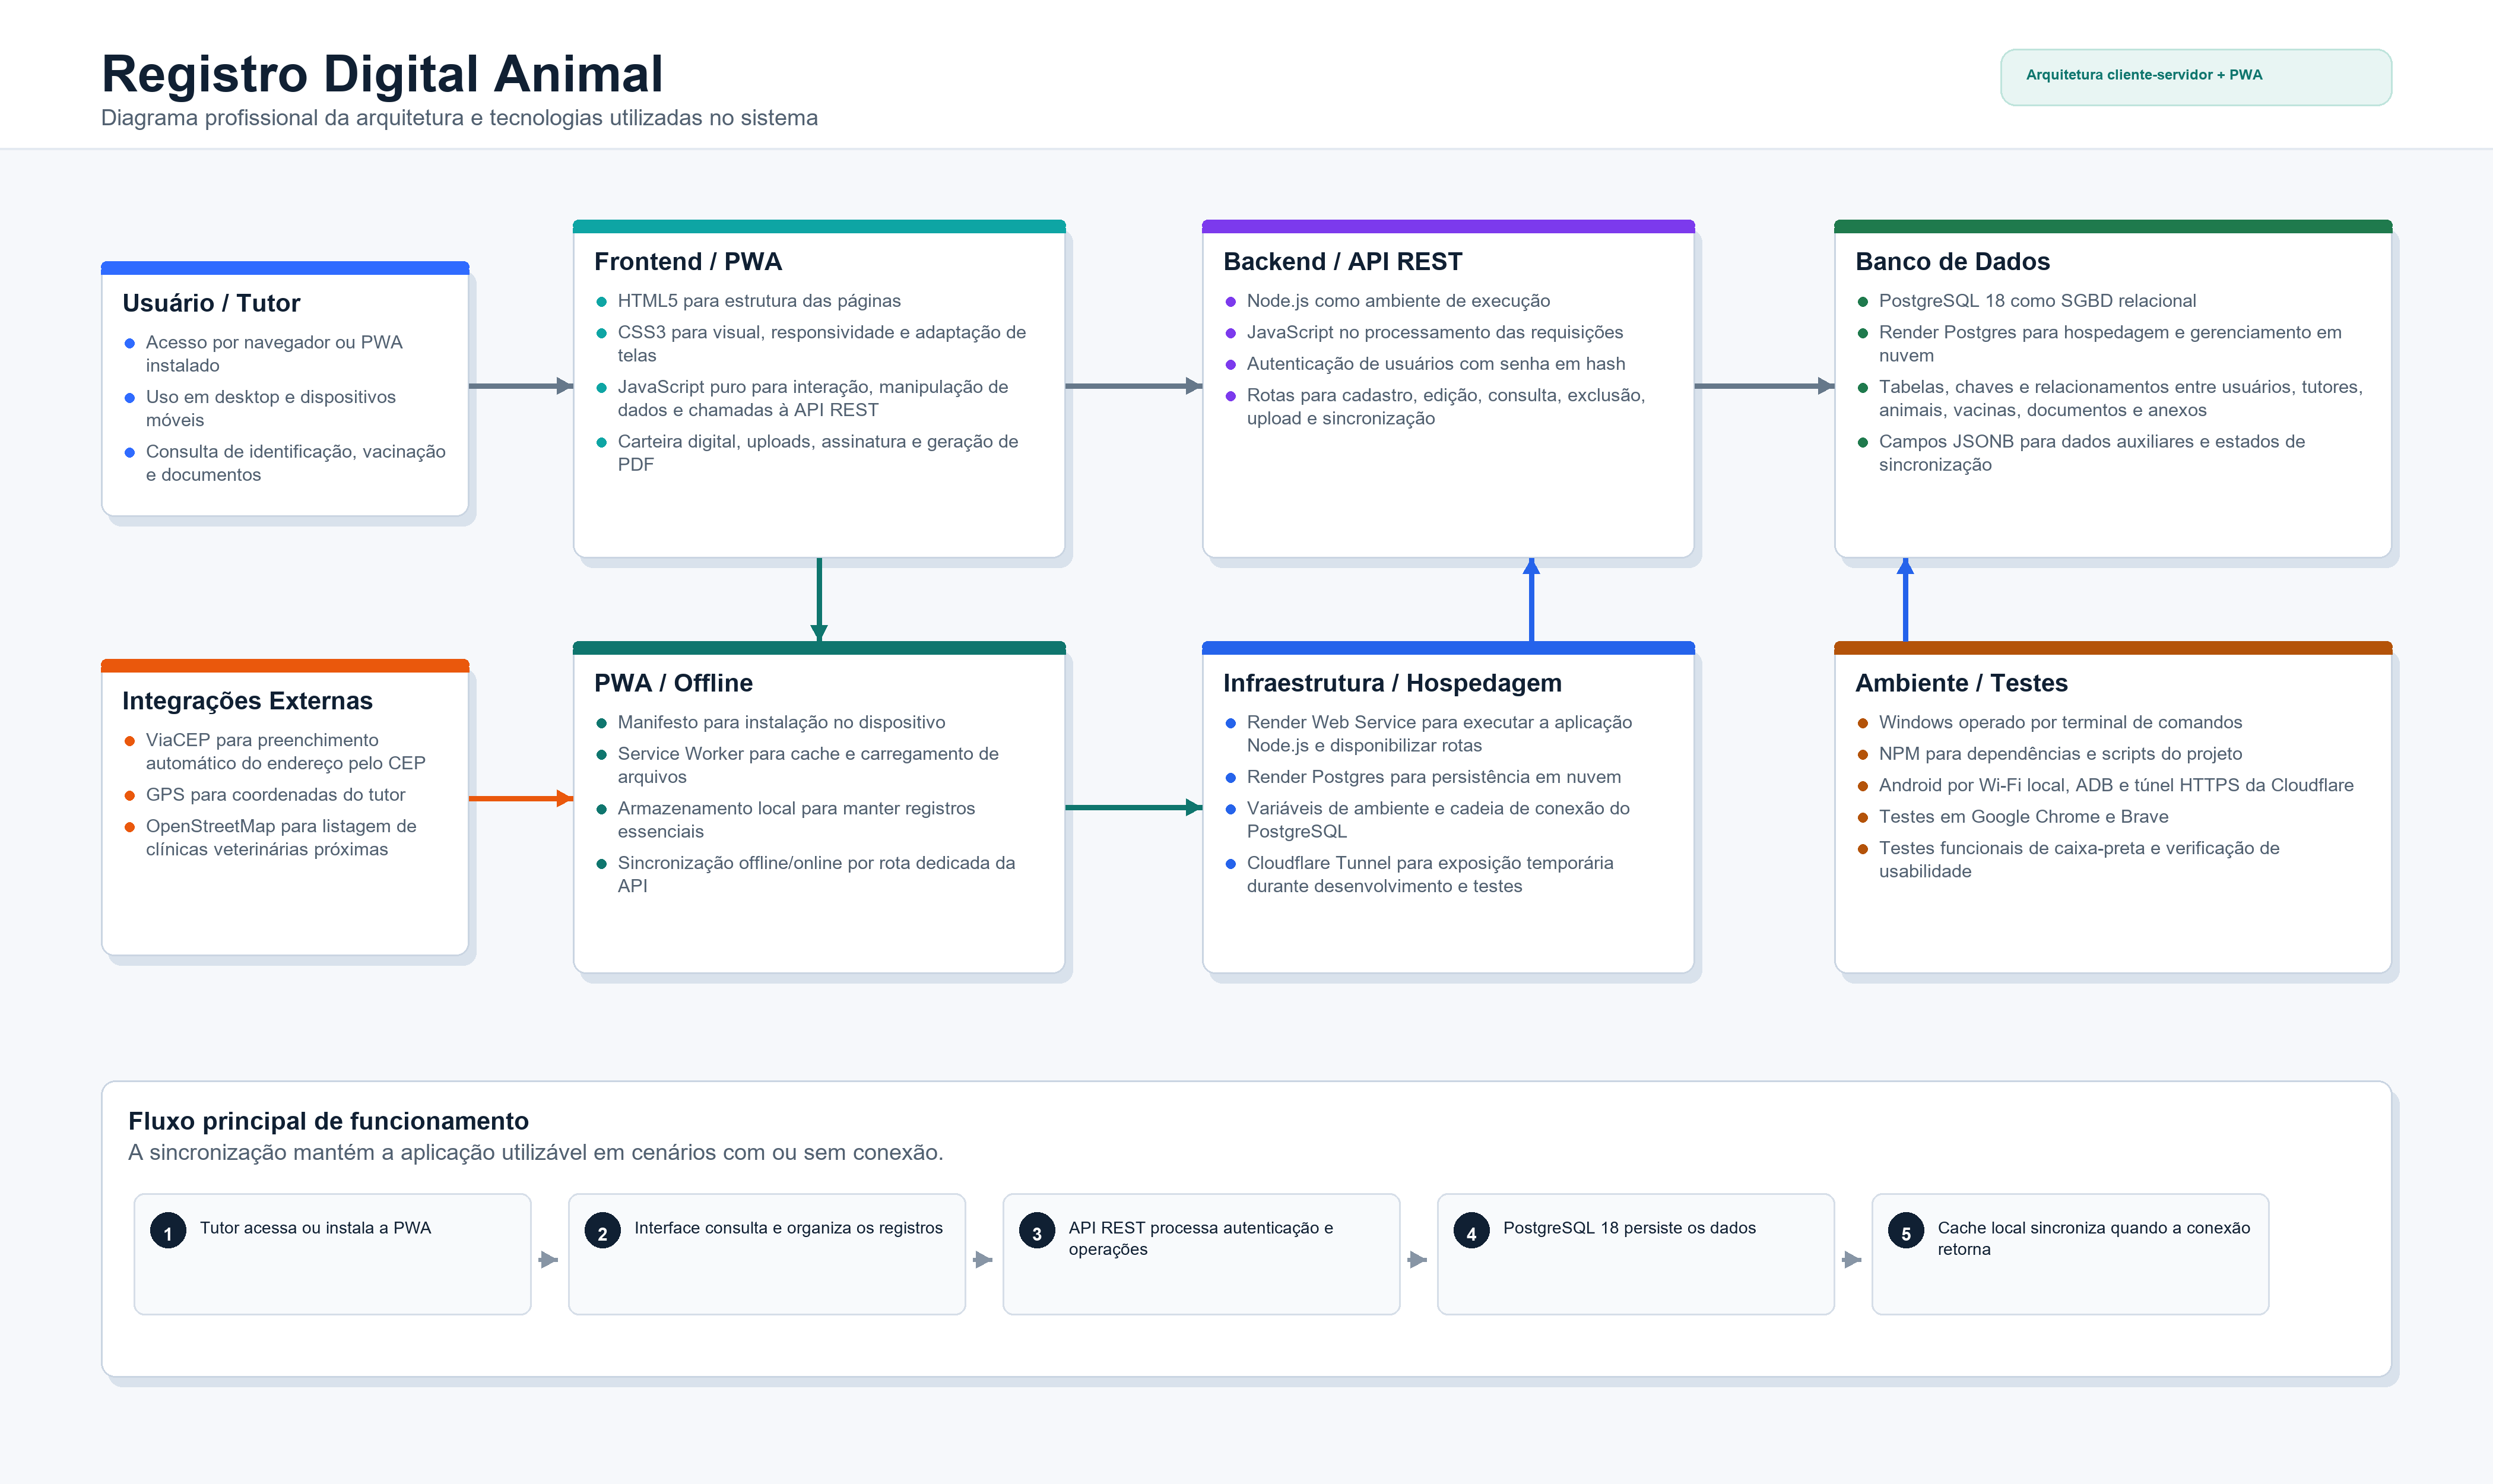
\includegraphics[width=\textwidth]{Figs/Registro_Digital_Animal_Diagrama.png}

\vspace{-0.2cm}
\begin{minipage}{\textwidth}
\footnotesize\raggedright Fonte: Elaborado pelo autor.
\end{minipage}
\end{figure}

As integrações externas incluem a API ViaCEP, para preenchimento automático de endereços, e os recursos de GPS e OpenStreetMap, para localizar clínicas veterinárias próximas ao tutor. No desenvolvimento e nos testes, foram usados Windows, os navegadores Google Chrome e Brave, dispositivos Android, rede local Wi-Fi, \textit{Android Debug Bridge} (ADB) e túnel HTTPS da Cloudflare.

A aplicação é composta por módulos de gerenciamento das informações do tutor e do animal. O módulo de usuários permite cadastro e autenticação via API, com senhas armazenadas em formato de \textit{hash}. O módulo de animais registra e edita os dados de identificação, incluindo o \textit{upload} de foto e o preenchimento automático do endereço a partir do CEP consultado na API ViaCEP, permanecendo sob responsabilidade do usuário o preenchimento do número e do complemento.

O sistema conta ainda com uma carteira digital do animal visualizável em formato frente e verso, recursos para captura de assinatura digital diretamente na aplicação, \textit{upload} de documentos do pet em imagem ou PDF e geração ou \textit{download} da carteira e de seus anexos compilados em PDF. Para auxiliar em situações de emergência e localização, a aplicação integra a geolocalização por GPS do tutor e os dados do OpenStreetMap para listar clínicas veterinárias próximas.

\subsubsection{Banco de Dados}

A Figura~\ref{fig:diagrama_banco_dados} apresenta um recorte de seis tabelas do núcleo cadastral da aplicação. A implementação contém ainda estruturas auxiliares para itens de viagem, avaliações, estado sincronizado, anexos, sincronizações em partes e eventos de uso, de modo que o diagrama não representa a totalidade do esquema. As seis estruturas representadas são:

\begin{itemize}
    \item \textbf{\texttt{pet\_app\_users}}: informações de cadastro e autenticação, incluindo nome, e-mail, telefone e \textit{hash} da senha;
    \item \textbf{\texttt{pet\_owners}}: dados do tutor vinculados ao usuário, como CPF, endereço, coordenadas de localização e contato de emergência;
    \item \textbf{\texttt{pet\_pets}}: identificação do animal, como espécie, raça, sexo, nascimento, peso, microchip, temperamento e alergias;
    \item \textbf{\texttt{pet\_vaccines}}: nome da vacina, dose, data de aplicação, data prevista da próxima dose, clínica, veterinário e lote;
    \item \textbf{\texttt{pet\_documents}}: título, categoria, data, validade e dados do anexo de cada documento;
    \item \textbf{\texttt{pet\_travel\_plans}}: destino, data da viagem, meio de transporte e animal selecionado.
\end{itemize}

\begin{figure}[htbp]
\captionsetup{
    justification=raggedright,
    singlelinecheck=false,
    format=hang
}
\caption{Recorte do núcleo cadastral do banco PostgreSQL da aplicação Registro Digital Animal}
\label{fig:diagrama_banco_dados}

\centering
\vspace{-0.2cm}

\adjustbox{
    Clip=0pt 0pt {.38\width} 0pt,
    width=.62\textwidth
}{
    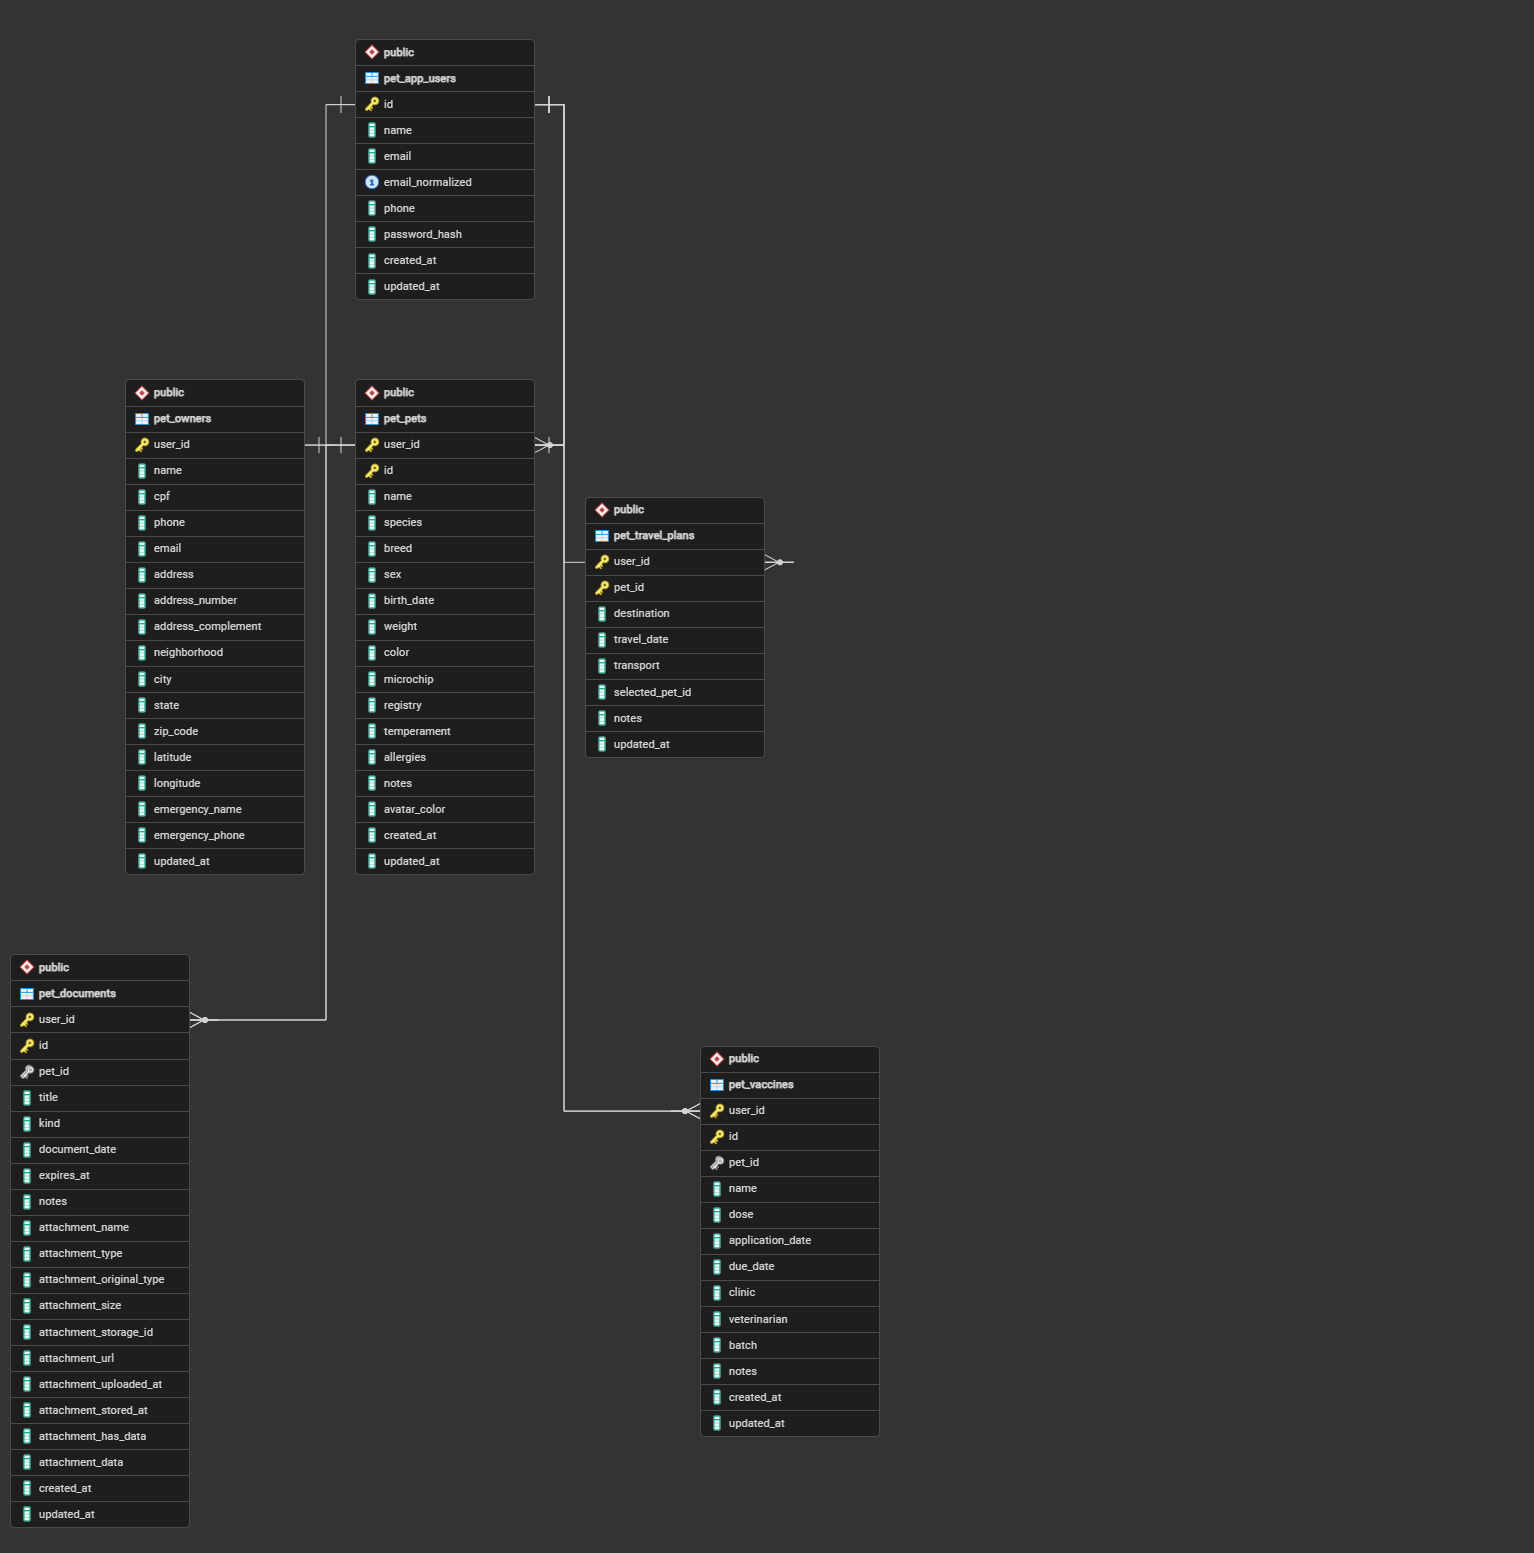
\includegraphics{Figs/Untitled.png}
}

\vspace{-0.2cm}
\begin{minipage}{\textwidth}
\footnotesize\raggedright
Fonte: Elaborado pelo autor.
\end{minipage}
\end{figure}

\subsection{Metodologia de Avaliação}

A avaliação compreendeu a verificação funcional de caixa-preta e a análise exploratória de retornos do setor veterinário. A verificação funcional comparou ações e resultados esperados; as observações sobre clareza das telas e navegação foram descritivas e não constituíram avaliação padronizada de usabilidade. A análise de retornos examinou utilidades percebidas e dificuldades relatadas, sem estimar aceitação populacional.

\subsubsection{Procedimento e cenários dos testes}

Os testes foram executados em computadores com Windows, nos navegadores Chrome e Brave, e em dispositivos Android, com acesso móvel por Wi-Fi local, depuração USB com ADB e túnel HTTPS da Cloudflare. Para cada cenário, comparou-se o comportamento observado ao esperado; a classificação \textit{Passou} correspondeu à execução da tarefa prevista e à manutenção dos dados envolvidos.

Foram organizados 15 cenários (F01 a F15), descritos na Tabela~\ref{tab:testes_funcionais}, abrangendo cadastro e autenticação, edição do animal, carteira e documentos, geolocalização, acesso móvel, consulta offline e sincronização. Em cada tarefa, verificaram-se o resultado esperado e a manutenção dos dados envolvidos, como vinculação de anexos ao pet, legibilidade da assinatura, consulta aos registros locais e persistência após restabelecer a conexão. Os registros não constituem bateria exaustiva de casos negativos, concorrência ou indisponibilidade de serviços, nem documentam tempos, número de tentativas ou avaliações independentes de usabilidade.

A escala de severidade de Nielsen classifica problemas de usabilidade por frequência, impacto e persistência \cite{nielsen1994}. Como não foi preservado um protocolo de julgamento independente desses fatores por cenário, não foram atribuídas notas de severidade, e a aprovação funcional foi mantida separada dos problemas relatados pelos participantes.

\subsubsection{Procedimento da pesquisa de campo}

O convite foi dirigido a clínicas, estabelecimentos e profissionais do setor animal, identificados pelo Google Maps em Criciúma e pela plataforma Casa dos Dados para outros municípios, em seleção não probabilística. A planilha de acompanhamento registrou 96 contatos, com convites entre 11 e 18 de setembro de 2026; predominaram localidades de Santa Catarina, mas um contato era de Fortaleza, e por isso o conjunto não foi tratado como exclusivamente catarinense. O contato ocorreu pelo WhatsApp, com apresentação do pesquisador; aos que aceitaram, foram enviados o endereço do aplicativo e um vídeo de orientação, solicitando opinião sobre a experiência de uso, informações ausentes e melhorias.

Os 96 contatos resultaram em 13 aceites, 80 sem resposta e três sem interesse. Aceitar o convite, receber o material, cadastrar-se e enviar uma avaliação foram tratados como eventos distintos. A planilha indicou dois feedbacks recebidos (21 de setembro e 7 de outubro de 2026); entre os demais aceites, dez ficaram pendentes e um registrou cadastro sem avaliação. O pesquisador informou ainda um terceiro retorno, armazenado no banco do Render e indisponível após a interrupção do serviço; ele não constava como recebido na planilha, e seu conteúdo não foi analisado. O corpus inicial foi composto pelos dois retornos preservados, identificados como R1 (avaliação estruturada salva pela aplicação, com notas e comentários) e R2 (relato textual livre de uma participante, que informou ter cadastrado seus animais), sem divulgação de nomes ou estabelecimentos.

No formulário, os campos gerais registraram satisfação com as informações da carteira e avaliação do aplicativo; os itens de concordância trataram da necessidade de melhoria e da utilidade de aprimoramentos em carteira, vacinação e viagens, sem serem interpretados como satisfação. Os comentários foram agrupados por conteúdo (organização e identificação; informação vacinal; viagens; localização de clínicas; atuação veterinária) e associados a R1 ou R2. Para esses dois retornos anteriores não foram produzidas estimativas estatísticas, e a categorização, feita por um único analista, não passou por concordância entre avaliadores.

Em 4 de novembro de 2026, foi realizada uma extração complementar das tabelas de avaliações e respostas da aplicação na Vercel. A unidade de análise foi definida como o último envio válido por conta, preservando a base original e evitando contar reenvios como novas avaliações. Os itens de concordância de 1 a 5 foram apresentados individualmente, acompanhados de medianas e médias exclusivamente descritivas; zeros nos campos gerais foram tratados como respostas ausentes, por estarem fora da escala. As contas dessa extração não foram vinculadas nominalmente aos convites anteriores. A análise manteve os dois conjuntos separados, categorizou os comentários por conteúdo e relacionou as solicitações às alterações do aplicativo. Não houve nova avaliação por participantes depois dessas alterações.

\section{RESULTADOS E DISCUSSÃO}

Esta seção apresenta os resultados funcionais, a análise dos dois retornos anteriores preservados e a coleta complementar de novembro. Cada fonte foi discutida conforme seu alcance: tarefas dos cenários definidos, relatos individuais, respostas estruturadas por conta e alterações técnicas posteriores. Os conjuntos não foram agregados como uma única amostra de participantes.

\subsection{Resultados dos cenários funcionais}

A Tabela~\ref{tab:testes_funcionais} apresenta os resultados dos 15 cenários. A classificação expressa o resultado funcional registrado, sem equivalência com medida de usabilidade.

\begin{table}[htbp]
\centering
\caption{Resultados registrados para os cenários funcionais do sistema}
\label{tab:testes_funcionais}
\par\vspace{4pt}
\small
\setlength{\tabcolsep}{4pt}
\renewcommand{\arraystretch}{1.1}
\begin{tabular}{@{}p{0.08\linewidth} p{\dimexpr0.76\linewidth-4\tabcolsep\relax} p{0.16\linewidth}@{}}
\hline
\textbf{ID} & \textbf{Cenário de teste avaliado} & \textbf{Resultado} \\
\hline
F01 & Cadastro de usuário e armazenamento de senha com \textit{hash} & Passou \\
F02 & Autenticação do usuário e controle de sessão na API REST & Passou \\
F03 & Cadastro e edição de perfil de animal com \textit{upload} de foto & Passou \\
F04 & Preenchimento automático de endereço via API ViaCEP a partir do CEP & Passou \\
F05 & Captura e salvamento de assinatura digital no formulário & Passou \\
F06 & Visualização interativa da carteira digital, com frente e verso & Passou \\
F07 & \textit{Upload} e vinculação de documentos clínicos em imagem ou PDF & Passou \\
F08 & Geração e exportação da carteira digital consolidada em PDF & Passou \\
F09 & Captura de coordenadas de geolocalização via GPS móvel & Passou \\
F10 & Consulta de clínicas veterinárias próximas via OpenStreetMap & Passou \\
F11 & Responsividade e navegação em \textit{desktop} nos navegadores Chrome e Brave & Passou \\
F12 & Acesso móvel em Android via Wi-Fi, ADB e túnel Cloudflare & Passou \\
F13 & Armazenamento e execução de \textit{cache} pelo \textit{Service Worker} & Passou \\
F14 & Acesso e consulta offline aos dados da carteira e das vacinas & Passou \\
F15 & Sincronização offline-online de registros no banco PostgreSQL & Passou \\
\hline
\end{tabular}
\par\vspace{2pt}
{\footnotesize\raggedright Fonte: Elaborado pelo autor.\par}
\end{table}

Os 15 cenários foram registrados como aprovados nas condições descritas. Os resultados abrangem os fluxos de cadastro, carteira e documentos (F01--F08), mobilidade e localização de clínicas (F09--F12), consulta offline e sincronização dos registros (F13--F15). A aprovação se restringe às tarefas previstas e aos ambientes avaliados: não demonstra ausência de falhas em outros cenários, confiabilidade em produção ou usabilidade generalizável. A consulta offline depende de dados previamente armazenados; serviços externos e envio ao servidor exigem conectividade.

\subsection{Análise dos retornos anteriores preservados da pesquisa de campo}

No acompanhamento inicial, o registro de recrutamento apresentou 13 aceites entre 96 contatos (13,5\%), e somente dois tiveram feedback marcado como recebido. Esses números descrevem o acompanhamento dos convites e não medem satisfação ou utilização efetiva. A Tabela~\ref{tab:recrutamento} resume as etapas documentadas.

\begin{table}[htbp]
\centering
\caption{Situação dos contatos e dos retornos no acompanhamento inicial}
\label{tab:recrutamento}
\small
\setlength{\tabcolsep}{5pt}
\renewcommand{\arraystretch}{1.1}
\begin{tabular}{@{}p{\dimexpr0.84\linewidth-2\tabcolsep\relax} r@{}}
\hline
\textbf{Etapa ou situação registrada} & \textbf{Quantidade} \\
\hline
Contatos com convite registrado & 96 \\
Aceitaram participar & 13 \\
Sem resposta ao convite & 80 \\
Não interessados & 3 \\
Aceites com feedback marcado como recebido & 2 \\
Aceites com feedback pendente & 10 \\
Aceite com cadastro, sem feedback, conforme observação & 1 \\
Retornos preservados incluídos na análise & 2 \\
Retorno adicional informado, indisponível e excluído & 1 \\
\hline
\end{tabular}
\par\vspace{2pt}
{\footnotesize\raggedright Fonte: Elaborado pelo autor.\par}
\end{table}

A Tabela~\ref{tab:resumo_qualitativo} relaciona os aspectos analisados aos registros que os sustentam. As descrições são menções individuais, sem indicação de prevalência entre profissionais veterinários.

\begin{table}[htbp]
\centering
\caption{Síntese dos comentários presentes nos dois retornos preservados}
\label{tab:resumo_qualitativo}
\small
\setlength{\tabcolsep}{4pt}
\renewcommand{\arraystretch}{1.1}
\begin{tabular}{@{}p{0.24\linewidth} p{\dimexpr0.66\linewidth-4\tabcolsep\relax} p{0.10\linewidth}@{}}
\hline
\textbf{Aspecto} & \textbf{Comentário ou sugestão registrada} & \textbf{Fonte} \\
\hline
Identificação e preenchimento & Dificuldade para informar o peso de 16,3; valorização de informações mais detalhadas sobre o animal. & R1 \\
Registro de vacinas & Questionamento sobre a necessidade do campo de quantidade de aplicação, considerado assunto de análise veterinária. & R1 \\
Organização e consulta & Utilidade dos dados para preenchimento pelo tutor e comunicação das informações durante o atendimento; navegação descrita como fácil. & R2 \\
Identificação por microchip & Valorização do registro de microchip como informação útil em situações de resgate. & R2 \\
Planejamento de viagens & Área descrita como completa e útil para organização antecipada de documentos. & R2 \\
Localização de clínicas & Utilidade da busca de estabelecimentos próximos e sugestão de destacar os que atendem 24 horas. & R2 \\
Atuação veterinária & Sugestão de área profissional com identificação pelo registro de conselho, consulta por microchip e registros de atendimento. & R2 \\
\hline
\end{tabular}
\par\vspace{2pt}
{\footnotesize\raggedright Fonte: Elaborado pelo autor a partir dos retornos preservados.\par}
\end{table}

Em R1, os campos gerais apresentaram nota 5 para as informações da carteira e nota 4 para a avaliação do aplicativo, em escala de 1 a 5; por pertencerem a um único retorno, não foram tratadas como média de satisfação. A dificuldade com peso decimal apareceu no exemplo de um animal com 16,3, registrado como 16 porque o valor exato não foi aceito na interação descrita. O achado evidencia uma limitação percebida no preenchimento, sem permitir atribuir sua causa ao navegador, à versão do aplicativo ou à validação de um campo específico. O comentário sobre a quantidade de aplicação indica a necessidade de revisar a clareza e a pertinência dos dados do módulo de vacinação, considerando a distinção entre registro pelo tutor e avaliação profissional.

R2 destacou a organização das informações e a facilidade de localizá-las, e considerou úteis os dados de identificação, o registro de microchip, o planejamento de viagens e a busca de clínicas próximas. A sugestão de destacar estabelecimentos 24 horas indica que a proximidade, isoladamente, pode ser insuficiente em situação de urgência, sem comprovação de redução do tempo de atendimento ou melhoria de desfechos clínicos. A sugestão de uma área veterinária, com consulta por microchip e registros de atendimento, amplia o problema para o compartilhamento de informações entre tutores e profissionais e exigiria investigar responsabilidades, autorização de acesso e verificação de identidade profissional; a menção a um número de conselho, por si só, não demonstra mecanismo suficiente de validação. Foi mantida como possibilidade de investigação, e não como funcionalidade entregue. Nesses dois retornos anteriores, não foram identificados comentários que comprovem aceitação do funcionamento offline, da exportação em PDF ou de notificações de revacinação; esses recursos foram descritos na avaliação técnica, e sua apreciação pelos participantes não foi presumida.

\subsection{Avaliações estruturadas registradas em novembro de 2026}
\label{sec:feedbacks_novembro}

A consulta complementar de 4 de novembro de 2026 relacionou as avaliações do Prisma Postgres na Vercel às respostas de cada pergunta pela chave composta de usuário e avaliação. Foram encontrados cinco envios de quatro contas. Dois eram idênticos, pertenciam à mesma conta e foram registrados com aproximadamente 15 segundos de diferença. Manteve-se apenas o mais recente dessa conta na análise, sem excluir registros do banco. O recorte contém quatro avaliações, uma por conta, identificadas como N1 a N4 em ordem cronológica, totalizando 24 respostas às seis afirmações de concordância.

Os envios selecionados ocorreram entre 15h15 e 15h29, no horário de Brasília; a base registra UTC. Essa proximidade não demonstra duração ou condições equivalentes de uso. Conta distinta não comprova participante independente: não foram estabelecidos profissão, município ou vínculo com os 13 aceites anteriores. Os novos registros não foram somados aos dois retornos preservados para anunciar seis participantes ou recalcular a taxa de resposta. Nomes, e-mails e identificadores técnicos foram omitidos.

\subsubsection{Escalas e tratamento das respostas}

O formulário possui dois campos gerais e seis afirmações, com concordância de 1 (discordo totalmente) a 5 (concordo totalmente), sendo 3 a posição neutra. Discordar de uma necessidade de melhoria difere de discordar da utilidade de uma sugestão; portanto, os itens não foram somados em um índice de satisfação ou usabilidade.

Nos dois campos gerais, N1 e N2 atribuíram nota 5, N4 atribuiu 4 e N3 apresentou zero. Como zero está fora da escala, foi tratado como resposta ausente nesses campos, mantendo-se os itens válidos de N3. Cada campo geral teve três notas válidas, com média descritiva 4,67 e mediana 5. A Tabela~\ref{tab:likert_novembro} apresenta as respostas de concordância individualmente, com médias descritivas e medianas, sem inferência populacional.

\begin{table}[htbp]
\centering
\caption{Respostas às afirmações de concordância, após seleção por conta}
\label{tab:likert_novembro}
\small
\setlength{\tabcolsep}{4pt}
\renewcommand{\arraystretch}{1.15}
\begin{tabular}{@{}p{\dimexpr0.53\linewidth-8\tabcolsep\relax}rrrrrr@{}}
\hline
\textbf{Afirmação resumida} & \textbf{N1} & \textbf{N2} & \textbf{N3} & \textbf{N4} & \textbf{Média} & \textbf{Med.} \\
\hline
Carteirinha precisa de informações mais claras e completas & 1 & 2 & 2 & 4 & 2,25 & 2 \\
Vacinas precisam apresentar melhor datas, clínica e situação & 1 & 2 & 2 & 2 & 1,75 & 2 \\
Viagens precisam organizar melhor checklist e documentos & 1 & 1 & 1 & 1 & 1,00 & 1 \\
Mais campos opcionais na carteirinha ajudariam na identificação & 2 & 2 & 4 & 4 & 3,00 & 3 \\
Alertas, filtros e destaque para vacinas atrasadas seriam úteis & 1 & 4 & 5 & 5 & 3,75 & 4,5 \\
Checklist por pet com dados e lembretes ajudaria no planejamento & 1 & 4 & 5 & 5 & 3,75 & 4,5 \\
\hline
\end{tabular}
\par\vspace{2pt}
{\footnotesize\raggedright Fonte: Elaborado pelo autor a partir das avaliações consultadas em 4 de novembro de 2026. Cada linha possui quatro respostas. Médias são sínteses descritivas de itens ordinais, acompanhadas das respostas individuais e medianas.\par}
\end{table}

Os quatro registros discordaram totalmente de que a organização de viagens precisava melhorar, mas três concordaram parcial ou totalmente com a utilidade de checklist por pet; uma conta discordou totalmente dessa sugestão. O mesmo padrão ocorreu para alertas de vacinas, com notas 4, 5 e 5 nos registros favoráveis e nota 1 no restante. Assim, baixa concordância com uma deficiência geral pode coexistir com interesse em incrementos. Para campos opcionais da carteira, houve duas discordâncias parciais e duas concordâncias parciais. Não foram realizados testes de significância ou avaliação psicométrica, nem atribuída severidade de Nielsen às notas: concordância com uma sugestão e severidade observada são medidas distintas.

\subsubsection{Comentários e transformação em requisitos}

N1 não acrescentou comentários. N2 solicitou alertas de vencimento e valorizou a preparação antecipada de viagens. N3 pediu que todas as vacinas vencidas fossem apresentadas; nos demais campos, informou não ter sugestões. N4 propôs resumir as pendências com dois nomes e a quantidade restante, selecionar vários pets para viajar, escolher entre checklist geral ou individual e acrescentar itens para necessidades específicas. Considerou úteis os alertas e avaliou novos campos de identificação como uma possibilidade sem necessidade extrema.

A categorização considerou o conteúdo, mesmo quando preenchido em campo associado a outro assunto: a solicitação de N3 sobre vacinas, por exemplo, estava em comentário da carteirinha. A priorização relacionou pedidos específicos às tarefas existentes, nas frentes de visibilidade dos prazos, síntese de pendências e flexibilidade de viagens. A Tabela~\ref{tab:rastreabilidade_feedbacks} apresenta essa relação, sem pressupor que todos os usuários tenham as mesmas necessidades.

\begin{table}[htbp]
\centering
\caption{Rastreabilidade entre comentários e alterações do aplicativo}
\label{tab:rastreabilidade_feedbacks}
\small
\setlength{\tabcolsep}{4pt}
\renewcommand{\arraystretch}{1.15}
\begin{tabular}{@{}p{\dimexpr0.28\linewidth-2\tabcolsep\relax}p{\dimexpr0.62\linewidth-2\tabcolsep\relax}p{0.10\linewidth}@{}}
\hline
\textbf{Necessidade relatada} & \textbf{Alteração implementada} & \textbf{Fonte} \\
\hline
Lembrar vencimentos & Central de avisos de vacinas e documentos, com vencidos, próximos 30 dias, filtros por categoria e acesso ao registro. & N2, N4 \\
Mostrar todas as vacinas vencidas & Listagem individual das pendências e síntese na carteira com quantidade, dois nomes e indicação das demais; ausência de registros não aparece como situação em dia. & N3, N4 \\
Preparar futuras viagens & Documentos do pet reunidos na tela de viagem e avisos de viagens nos próximos 30 dias com checklist pendente. & N2 \\
Organizar vários pets & Seleção de acompanhantes no plano de viagem, com escolha entre listas individuais e checklist compartilhado para o grupo selecionado. & N4 \\
Contemplar necessidades específicas & Inclusão e remoção de itens adicionais do checklist e campo de anotações; marcações compartilhadas se propagam somente ao grupo. & N4 \\
\hline
\end{tabular}
\par\vspace{2pt}
{\footnotesize\raggedright Fonte: Elaborado pelo autor. As alterações representam resposta de desenvolvimento aos comentários, sem comprovação de melhora de usabilidade após a mudança.\par}
\end{table}

Os avisos são calculados dentro do app a partir das datas e dos dados disponíveis no dispositivo; não há envio ao sistema operacional com o aplicativo fechado. Dependem da completude dos registros, da data do aparelho e da sincronização entre dispositivos.

Seis testes automatizados com dados fictícios verificaram regras de datas, contagem e listagem de vacinas vencidas, seleção de avisos de documentos e viagens, propagação de marcações e remoções no grupo e preservação das listas em JSON. Esses testes verificam regras técnicas; não equivalem a reavaliação por participantes nem comprovam satisfação com a versão modificada, aumento da adesão vacinal ou redução de esquecimentos.

\subsection{Limitações e ameaças à validade}

A avaliação funcional se limitou aos cenários e ambientes descritos, sem cobertura exaustiva de entradas inválidas, falhas de serviços externos, conflitos entre dispositivos ou perda de conexão durante o envio de anexos. A ausência de medidas de tempo, repetição e comparação com outra solução restringe conclusões sobre desempenho e facilidade de uso, e a observação feita no contexto de desenvolvimento pode favorecer a familiaridade com os fluxos, reduzindo a identificação de dificuldades de novos usuários.

Na pesquisa de campo, a seleção por conveniência, os dois retornos anteriores, a caracterização incompleta dos respondentes, a perda de um retorno e a categorização por um único analista limitam a comparação entre participantes. Na coleta complementar, quatro contas não comprovam quatro participantes independentes, e sua correspondência com os contatos anteriores não foi estabelecida. A concentração dos envios em um mesmo dia, a repetição por uma conta e a ausência de resposta válida aos campos gerais em outra exigiram explicitar critérios de seleção e denominadores. A pequena quantidade de avaliações e a ausência de reavaliação após as alterações impedem atribuir melhoria de usabilidade às funcionalidades adicionadas. A diferença entre aceites e retornos preservados introduz viés de não resposta: as percepções disponíveis podem não representar quem não respondeu ou aceitou sem avaliar. Os resultados não demonstram redução do uso de registros físicos, aumento de adesão à vacinação ou superioridade em relação a aplicativos existentes, e a pesquisa não avaliou a autenticação de autoria da assinatura capturada nem a aceitação documental do PDF por terceiros. Essas limitações delimitam a contribuição como desenvolvimento de um artefato e avaliação exploratória de seu funcionamento e de necessidades percebidas.

\section{CONCLUSÃO}

O trabalho desenvolveu a aplicação multiplataforma Registro Digital Animal para organizar e consultar identificação, vacinação e documentos clínicos de animais de estimação. O objetivo foi atendido no âmbito dos módulos e cenários descritos: cadastro de tutores e pets, carteira digital, documentos, registros vacinais e consulta em computadores e dispositivos móveis, com acesso a dados previamente armazenados e sincronização posterior.

Os 15 cenários funcionais foram registrados como aprovados nas condições avaliadas, sem comprovar ausência de falhas ou usabilidade generalizável. Os dois retornos anteriores indicaram utilidade na organização dos dados e dificuldades de preenchimento. A coleta complementar reuniu quatro avaliações, uma por conta, após desconsiderar um envio repetido. Os comentários orientaram avisos internos, resumo de vacinas vencidas, documentos na tela de viagens e checklists individuais ou compartilhados com itens adicionais. Seis testes automatizados verificaram regras dessas alterações; sua satisfação e facilidade de uso não foram reavaliadas por participantes.

A contribuição é o artefato e a rastreabilidade entre necessidades relatadas e alterações implementadas. O alcance é limitado pela seleção não probabilística, pelo conjunto reduzido de registros, pela caracterização incompleta das contas, pela perda de um retorno anterior e pela ausência de comparação com documentos físicos. A redução da dependência do papel permaneceu como benefício pretendido, sem mensuração. A experiência reforçou a necessidade de preservar os dados de avaliação e distinguir funcionamento técnico, clareza da interface e utilidade percebida.

Como trabalhos futuros, propõem-se avaliações com tutores e veterinários de diferentes perfis, comparação do tempo de localização e da completude dos registros com a documentação física e acompanhamento longitudinal dos prazos vacinais. Também devem ser investigados conectividade intermitente, edições concorrentes, recuperação de dados e participação profissional, considerando autorização de acesso e confiabilidade das informações.

\bibliographystyle{abntex2-alf}
\renewcommand{\refname}{REFERÊNCIAS}
\bibliography{referencias}

\end{document}